\section{Use case diagrams}
%Tutte le volte che è stato utilizzato bug l'abbiamo considerato come issue generica 
%Le notifiche erano presenti sia in F4 che in F6 e abbiamo creato un use case a parte per la visualizzazione di queste
%Aggiunto use case per il login di utente esterno
%Aggiunta di commento allo use in figura 4 delle issue per indicare che queste possano essere suggerite dal sistema come da F14
%modificare figura 5 in draw.io eliminare commento e aggiungere al commento in figura 4 il riferimento all'invio di notifica in caso di assegnazione di issue

\begin{figure}[H]\label{LoginUseCase}
    \centering
    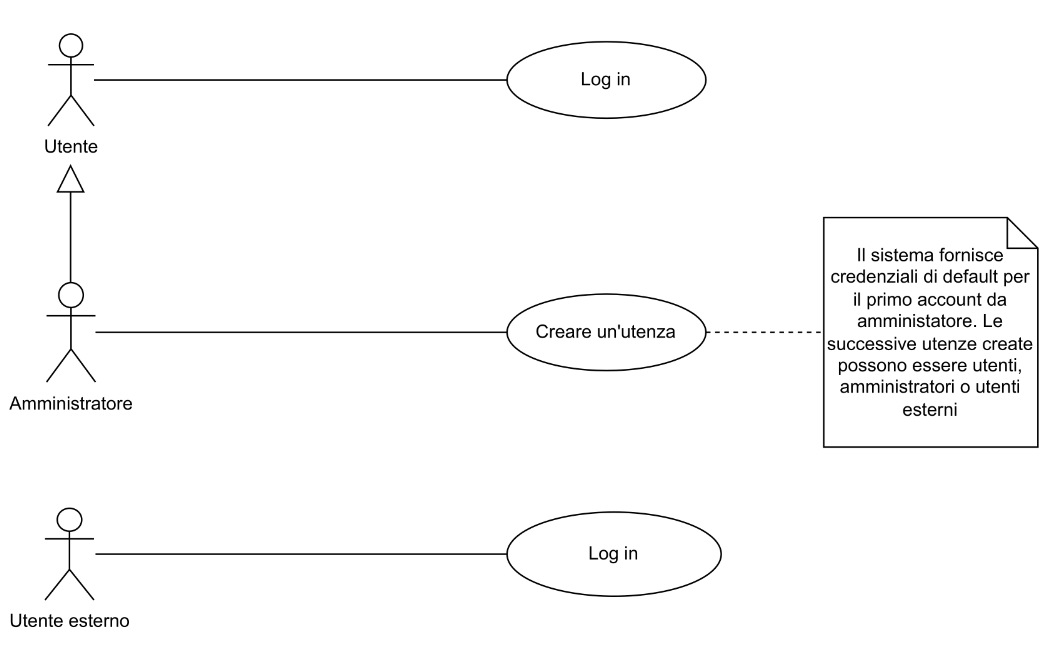
\includegraphics[width=0.8\linewidth]{src/useCaseDiagrams/LoginUseCase.png}
    \caption{Login use case diagram}
\end{figure}

\vspace{2cm}

\begin{figure}[H]\label{SegnalazioneUseCase}
    \centering
    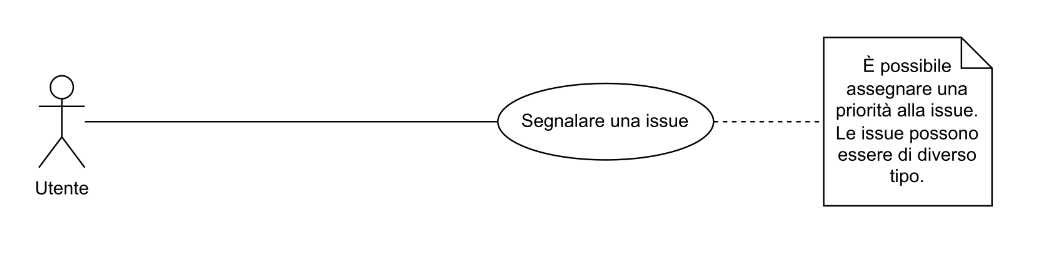
\includegraphics[width=0.8\linewidth]{src/useCaseDiagrams/SegnalaIssueUseCase.png}
    \caption{Segnalazione issue use case diagram}
\end{figure}

\vspace{2cm}

\begin{figure}[H]\label{RiepilogoIssueUseCase}
    \centering
    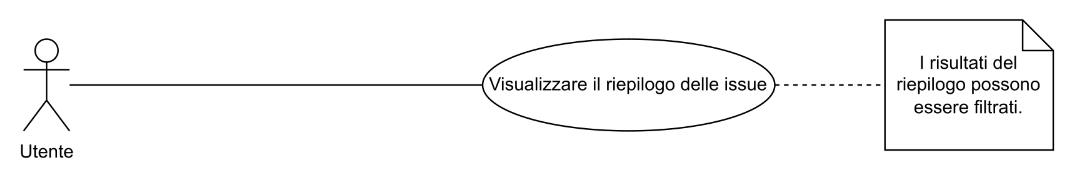
\includegraphics[width=0.8\linewidth]{src/useCaseDiagrams/VisualizzaRiepilogoUseCase.png}
    \caption{Visualizzazione riepilogo issue use case diagram}
\end{figure}

\vspace{2cm}

\begin{figure}[H]\label{AssegnazioneBugUseCase}
    \centering
    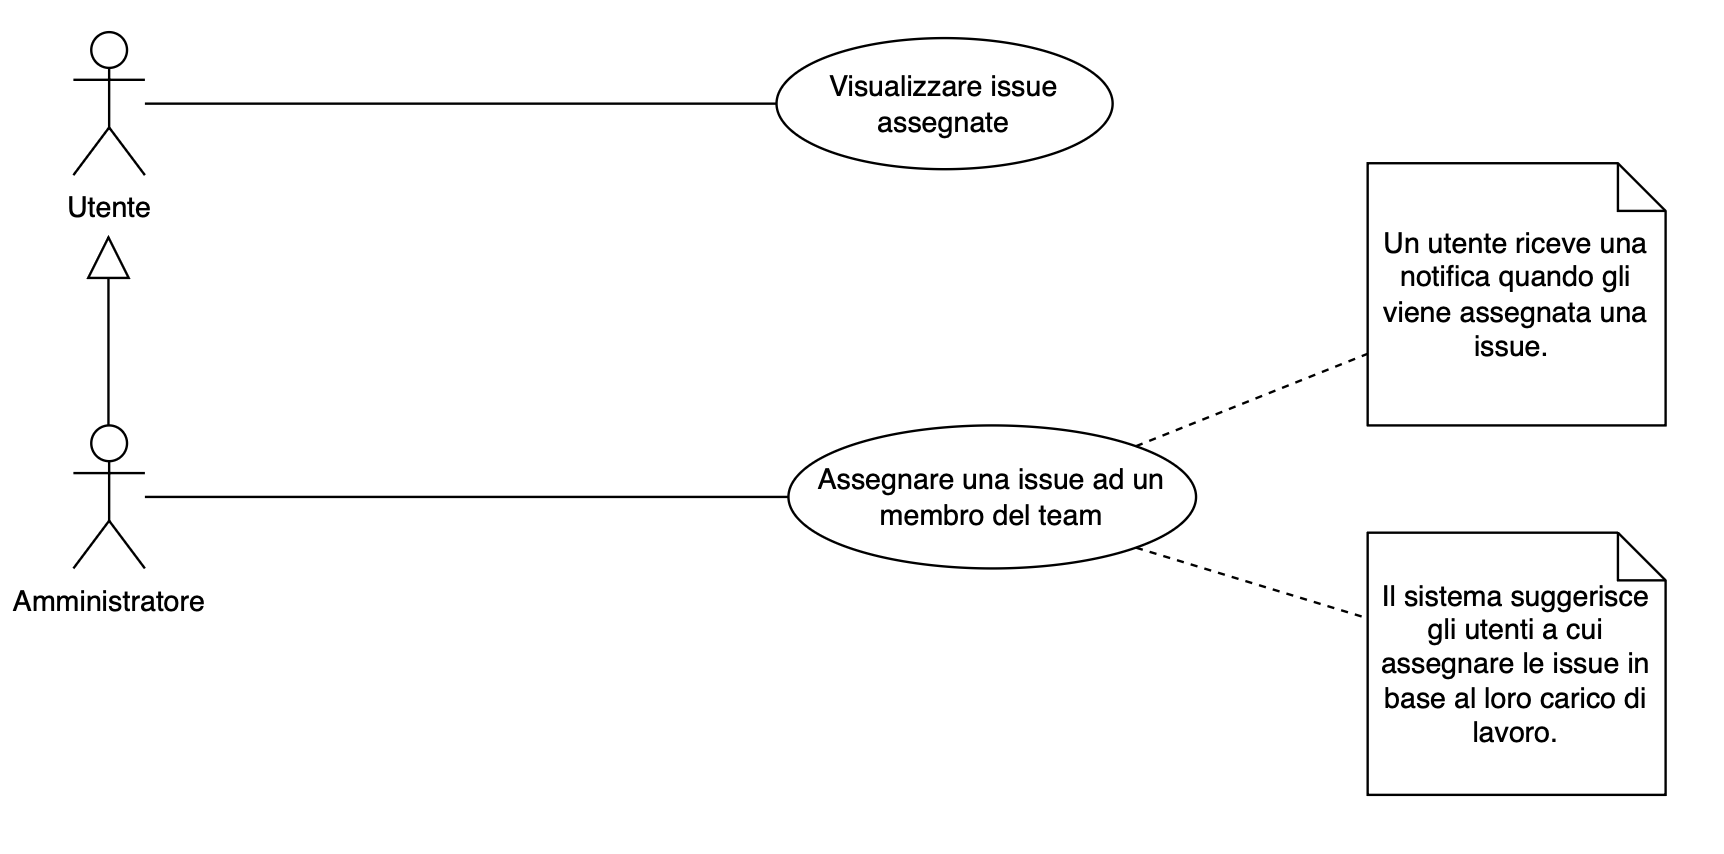
\includegraphics[width=0.8\linewidth]{src/useCaseDiagrams/AssegnaBugUseCase.png}
    \caption{Assegnazione issue use case diagram}
\end{figure}

\vspace{2cm}

\begin{figure}[H]\label{VisualizzaNotificheUseCase}
    \centering
    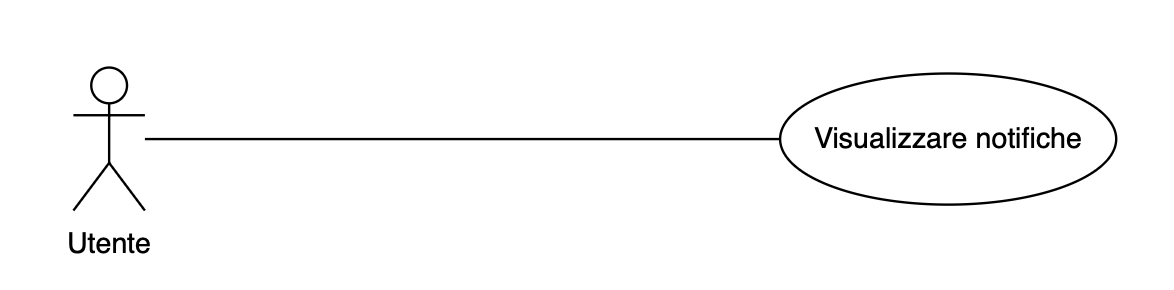
\includegraphics[width=0.8\linewidth]{src/useCaseDiagrams/VisualizzaNotificheUseCase.png}
    \caption{Visualizzazione notifiche use case diagram}
\end{figure}

\vspace{2cm}

\begin{figure}[H]\label{InserireCommentiUseCase}
    \centering
    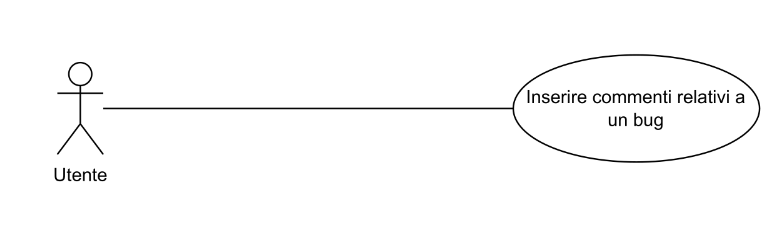
\includegraphics[width=0.8\linewidth]{src/useCaseDiagrams/InserireCommentiUseCase.png}
    \caption{Inserimento commenti use case diagram}
\end{figure}

\vspace{2cm}

\begin{figure}[H]\label{ModificaStatoUseCase}
    \centering
    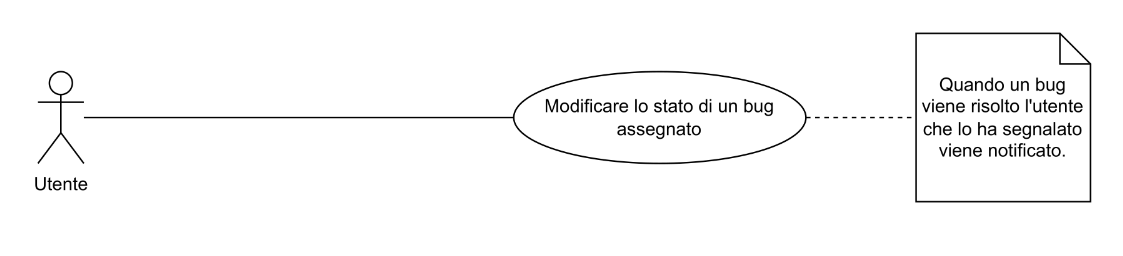
\includegraphics[width=0.9\linewidth]{src/useCaseDiagrams/ModificareStatoBugUseCase.png}
    \caption{Modificare stato di una issue use case diagram}
\end{figure}

\vspace{2cm}

\begin{figure}[H]\label{VisualizzaDashboardUseCase}
    \centering
    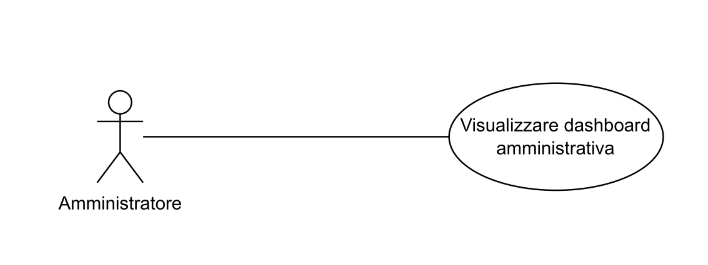
\includegraphics[width=0.7\linewidth]{src/useCaseDiagrams/VisualizzareDashboardUseCase.png}
    \caption{Visualizzazione dashboard use case diagram}
\end{figure}

\vspace{2cm}

\begin{figure}[H]\label{EsportareElencoUseCase}
    \centering
    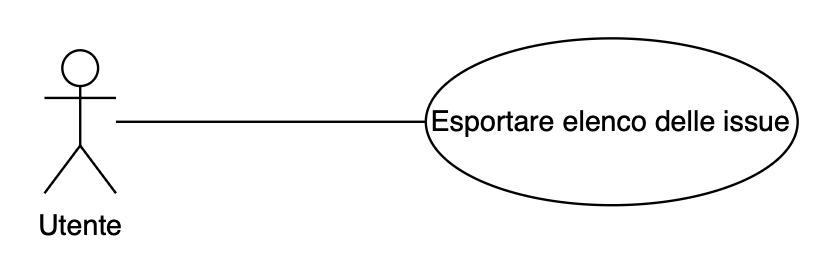
\includegraphics[width=0.5\linewidth]{src/useCaseDiagrams/EsportareElencoBugUseCase.png}
    \caption{Esportare elenco delle issue use case diagram}
\end{figure}

\vspace{2cm}

\begin{figure}[H]\label{ModificaBugUseCase}
    \centering
    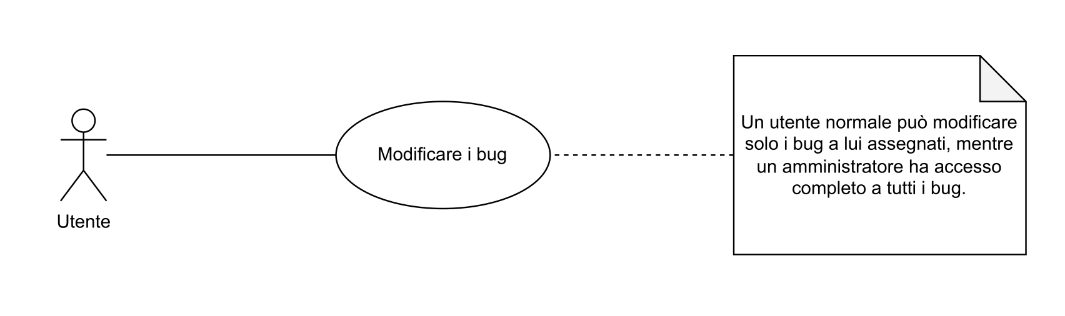
\includegraphics[width=0.8\linewidth]{src/useCaseDiagrams/ModificareBugUseCase.png}
    \caption{Modificare una issue use case diagram}
\end{figure}

\vspace{2cm}

\begin{figure}[H]\label{AssociazioneEtichettaUseCase}
    \centering
    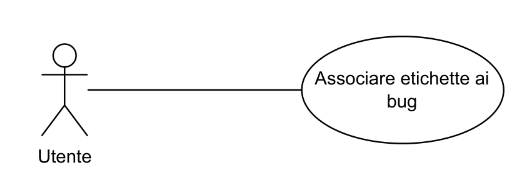
\includegraphics[width=0.5\linewidth]{src/useCaseDiagrams/AssociareEtichetteUseCase.png}
    \caption{Associare etichetta ad una issue use case diagram}
\end{figure}

\vspace{2cm}

\begin{figure}[H]\label{CercaBugUseCase}
    \centering
    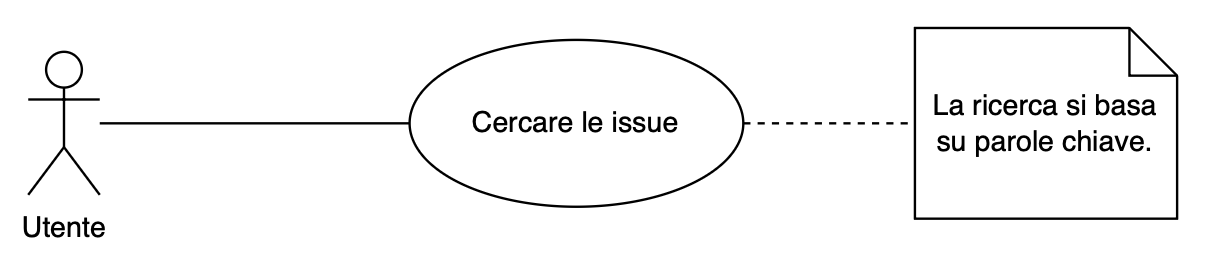
\includegraphics[width=0.8\linewidth]{src/useCaseDiagrams/CercareBugUseCase.png}
    \caption{Cercare una issue use case diagram}
\end{figure}

\vspace{2cm}

\begin{figure}[H]\label{VisualizzaCronologiaModificheUseCase}
    \centering
    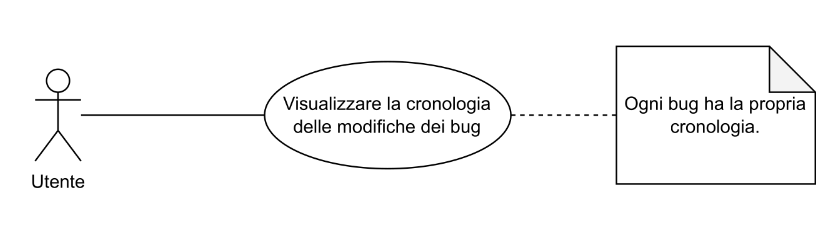
\includegraphics[width=0.8\linewidth]{src/useCaseDiagrams/VisualizzaCronologiaModificheUseCase.png}
    \caption{Visualizzazione cronologia modifiche issue use case diagram}
\end{figure}

\vspace{2cm}

\begin{figure}[H]\label{ArchiviareBugUseCase}
    \centering
    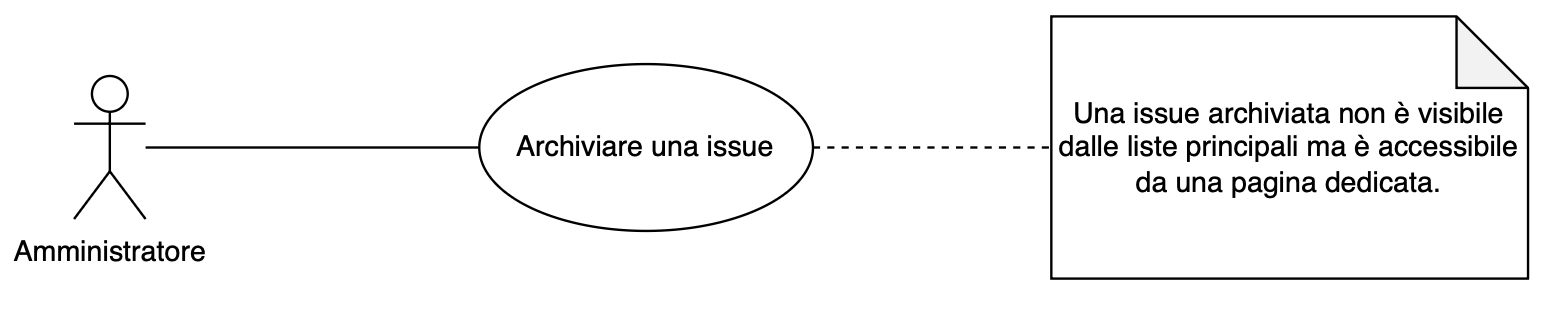
\includegraphics[width=0.8\linewidth]{src/useCaseDiagrams/ArchiviareBugUseCase.png}
    \caption{Archiviazione issue use case diagram}
\end{figure}

\vspace{2cm}

\begin{figure}[H]\label{VisualizzazioneBugCommentiUseCase}
    \centering
    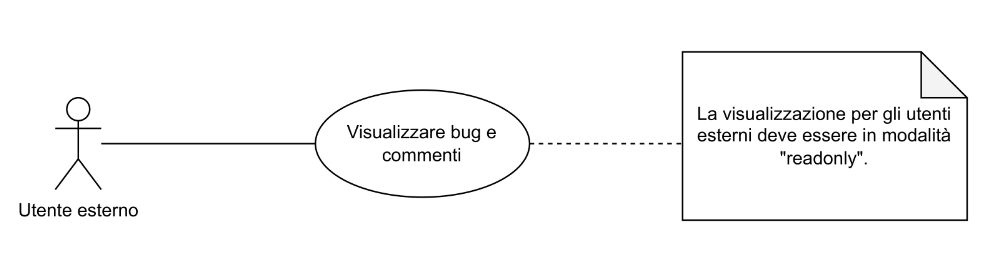
\includegraphics[width=0.8\linewidth]{src/useCaseDiagrams/VisualizzareBugCommentiUseCase.png}
    \caption{Visualizzazione "readonly" issue e commenti use case diagram}
\end{figure}

\vspace{2cm}

\begin{figure}[H]\label{ContrassegnaComeDuplicatoUseCase}
    \centering
    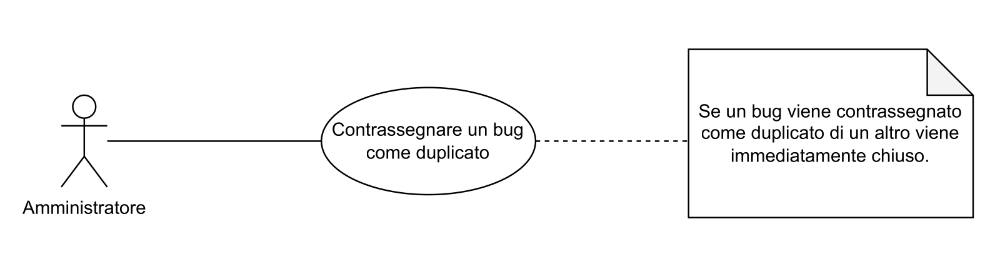
\includegraphics[width=0.8\linewidth]{src/useCaseDiagrams/ContrassegnaDuplicatiUseCase.png}
    \caption{Contrassegna una issue come duplicato use case diagram}
\end{figure}

\vspace{2cm}

\begin{figure}[H]\label{VisualizzaReportMensileUseCase}
    \centering
    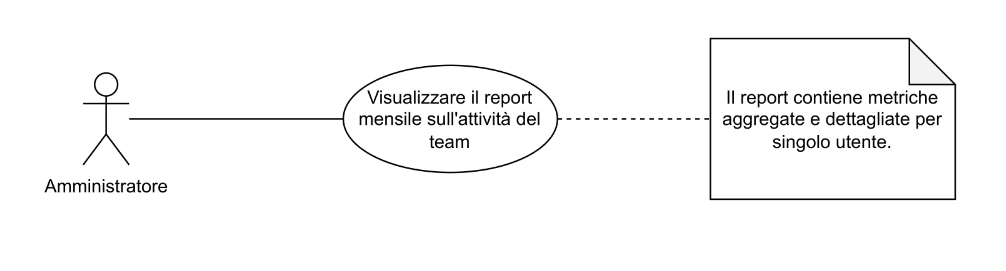
\includegraphics[width=0.8\linewidth]{src/useCaseDiagrams/VisualizzaReportMensileUseCase.png}
    \caption{Visualizzazione report mensile use case diagram}
\end{figure}

\vspace{2cm}

\begin{figure}[H]\label{ImpostaScadenzeUseCase}
    \centering
    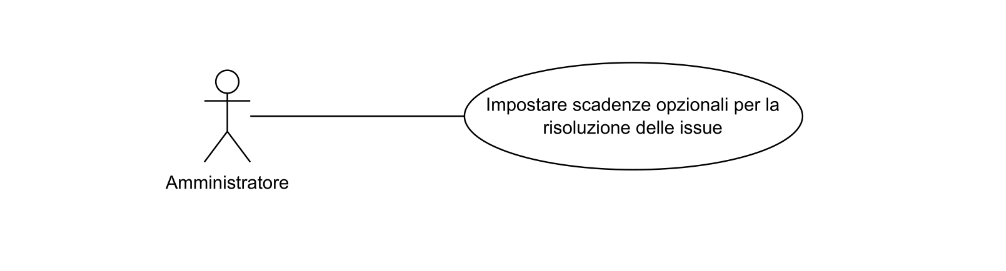
\includegraphics[width=0.9\linewidth]{src/useCaseDiagrams/ImpostaScadenzeUseCase.png}
    \caption{Imposta scadenze per la risoluzione di issue use case diagram}
\end{figure}